\begin{minipage}[b]{0.31\textwidth}\centering
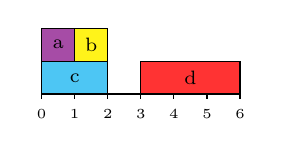
\begin{tikzpicture}[x=0.42cm,y=0.42cm,font=\scriptsize]
\draw[fill=cyan!70] (0,0) rectangle (2,1);\node at (1.0,0.5) {c};
\draw[fill=red!80] (3,0) rectangle (6,1);\node at (4.5,0.5) {d};
\draw[fill=violet!70] (0,1) rectangle (1,2);\node at (0.5,1.5) {a};
\draw[fill=yellow!90] (1,1) rectangle (2,2);\node at (1.5,1.5) {b};
\draw[thick] (0,0) -- (6,0);
\draw (0,0) -- (0,-0.15) node[below,font=\tiny] {0};
\draw (1,0) -- (1,-0.15) node[below,font=\tiny] {1};
\draw (2,0) -- (2,-0.15) node[below,font=\tiny] {2};
\draw (3,0) -- (3,-0.15) node[below,font=\tiny] {3};
\draw (4,0) -- (4,-0.15) node[below,font=\tiny] {4};
\draw (5,0) -- (5,-0.15) node[below,font=\tiny] {5};
\draw (6,0) -- (6,-0.15) node[below,font=\tiny] {6};
\end{tikzpicture}\\[2pt] $S_0$\end{minipage}\hfill
\begin{minipage}[b]{0.31\textwidth}\centering
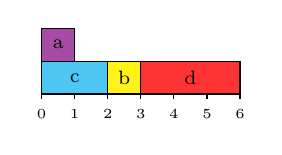
\begin{tikzpicture}[x=0.42cm,y=0.42cm,font=\scriptsize]
\draw[fill=cyan!70] (0,0) rectangle (2,1);\node at (1.0,0.5) {c};
\draw[fill=yellow!90] (2,0) rectangle (3,1);\node at (2.5,0.5) {b};
\draw[fill=red!80] (3,0) rectangle (6,1);\node at (4.5,0.5) {d};
\draw[fill=violet!70] (0,1) rectangle (1,2);\node at (0.5,1.5) {a};
\draw[thick] (0,0) -- (6,0);
\draw (0,0) -- (0,-0.15) node[below,font=\tiny] {0};
\draw (1,0) -- (1,-0.15) node[below,font=\tiny] {1};
\draw (2,0) -- (2,-0.15) node[below,font=\tiny] {2};
\draw (3,0) -- (3,-0.15) node[below,font=\tiny] {3};
\draw (4,0) -- (4,-0.15) node[below,font=\tiny] {4};
\draw (5,0) -- (5,-0.15) node[below,font=\tiny] {5};
\draw (6,0) -- (6,-0.15) node[below,font=\tiny] {6};
\end{tikzpicture}\\[2pt] $S_{1}$\end{minipage}\hfill
\begin{minipage}[b]{0.31\textwidth}\centering
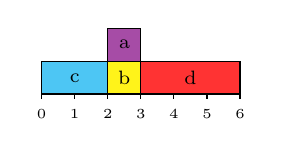
\begin{tikzpicture}[x=0.42cm,y=0.42cm,font=\scriptsize]
\draw[fill=cyan!70] (0,0) rectangle (2,1);\node at (1.0,0.5) {c};
\draw[fill=yellow!90] (2,0) rectangle (3,1);\node at (2.5,0.5) {b};
\draw[fill=red!80] (3,0) rectangle (6,1);\node at (4.5,0.5) {d};
\draw[fill=violet!70] (2,1) rectangle (3,2);\node at (2.5,1.5) {a};
\draw[thick] (0,0) -- (6,0);
\draw (0,0) -- (0,-0.15) node[below,font=\tiny] {0};
\draw (1,0) -- (1,-0.15) node[below,font=\tiny] {1};
\draw (2,0) -- (2,-0.15) node[below,font=\tiny] {2};
\draw (3,0) -- (3,-0.15) node[below,font=\tiny] {3};
\draw (4,0) -- (4,-0.15) node[below,font=\tiny] {4};
\draw (5,0) -- (5,-0.15) node[below,font=\tiny] {5};
\draw (6,0) -- (6,-0.15) node[below,font=\tiny] {6};
\end{tikzpicture}\\[2pt] $S_{2}$\end{minipage}\\[8pt]
\begin{minipage}[b]{0.31\textwidth}\centering
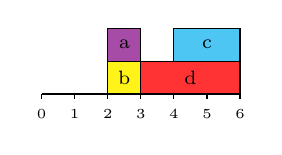
\begin{tikzpicture}[x=0.42cm,y=0.42cm,font=\scriptsize]
\draw[fill=yellow!90] (2,0) rectangle (3,1);\node at (2.5,0.5) {b};
\draw[fill=red!80] (3,0) rectangle (6,1);\node at (4.5,0.5) {d};
\draw[fill=violet!70] (2,1) rectangle (3,2);\node at (2.5,1.5) {a};
\draw[fill=cyan!70] (4,1) rectangle (6,2);\node at (5.0,1.5) {c};
\draw[thick] (0,0) -- (6,0);
\draw (0,0) -- (0,-0.15) node[below,font=\tiny] {0};
\draw (1,0) -- (1,-0.15) node[below,font=\tiny] {1};
\draw (2,0) -- (2,-0.15) node[below,font=\tiny] {2};
\draw (3,0) -- (3,-0.15) node[below,font=\tiny] {3};
\draw (4,0) -- (4,-0.15) node[below,font=\tiny] {4};
\draw (5,0) -- (5,-0.15) node[below,font=\tiny] {5};
\draw (6,0) -- (6,-0.15) node[below,font=\tiny] {6};
\end{tikzpicture}\\[2pt] $S_{3}$\end{minipage}\hfill
\begin{minipage}[b]{0.31\textwidth}\centering
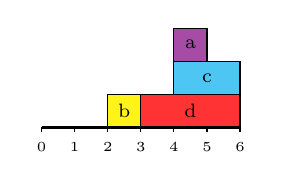
\begin{tikzpicture}[x=0.42cm,y=0.42cm,font=\scriptsize]
\draw[fill=yellow!90] (2,0) rectangle (3,1);\node at (2.5,0.5) {b};
\draw[fill=red!80] (3,0) rectangle (6,1);\node at (4.5,0.5) {d};
\draw[fill=cyan!70] (4,1) rectangle (6,2);\node at (5.0,1.5) {c};
\draw[fill=violet!70] (4,2) rectangle (5,3);\node at (4.5,2.5) {a};
\draw[thick] (0,0) -- (6,0);
\draw (0,0) -- (0,-0.15) node[below,font=\tiny] {0};
\draw (1,0) -- (1,-0.15) node[below,font=\tiny] {1};
\draw (2,0) -- (2,-0.15) node[below,font=\tiny] {2};
\draw (3,0) -- (3,-0.15) node[below,font=\tiny] {3};
\draw (4,0) -- (4,-0.15) node[below,font=\tiny] {4};
\draw (5,0) -- (5,-0.15) node[below,font=\tiny] {5};
\draw (6,0) -- (6,-0.15) node[below,font=\tiny] {6};
\end{tikzpicture}\\[2pt] $S_{4}$\end{minipage}\hfill
\begin{minipage}[b]{0.31\textwidth}\centering
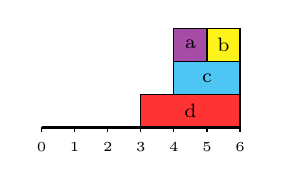
\begin{tikzpicture}[x=0.42cm,y=0.42cm,font=\scriptsize]
\draw[fill=red!80] (3,0) rectangle (6,1);\node at (4.5,0.5) {d};
\draw[fill=cyan!70] (4,1) rectangle (6,2);\node at (5.0,1.5) {c};
\draw[fill=violet!70] (4,2) rectangle (5,3);\node at (4.5,2.5) {a};
\draw[fill=yellow!90] (5,2) rectangle (6,3);\node at (5.5,2.5) {b};
\draw[thick] (0,0) -- (6,0);
\draw (0,0) -- (0,-0.15) node[below,font=\tiny] {0};
\draw (1,0) -- (1,-0.15) node[below,font=\tiny] {1};
\draw (2,0) -- (2,-0.15) node[below,font=\tiny] {2};
\draw (3,0) -- (3,-0.15) node[below,font=\tiny] {3};
\draw (4,0) -- (4,-0.15) node[below,font=\tiny] {4};
\draw (5,0) -- (5,-0.15) node[below,font=\tiny] {5};
\draw (6,0) -- (6,-0.15) node[below,font=\tiny] {6};
\end{tikzpicture}\\[2pt] $S_{5}$\end{minipage}\\[8pt]